\section{Planning with Clearance Value Annotations}
\label{aha:annotations}
In order to meet our stated goal of building a planner able to solve problems involving many degrees of heterogeneity we must first consider how to create an information-rich representation of the environment. Superficially, this problem appears trivial; given a grid-based representation of the map, any tile which is not an obstacle is traversable for some agent. Even in complex non-homogenous environments we can easily build a planner which takes into consideration an agent's terrain-traversal capability and limits the search space to locations the agent is able to cross.
The problem becomes more difficult when we introduce variability in the size of the agent as each location in a grid environment has a fixed size; if some agents are larger than others they could occupy several tiles at once and the performance of our planner would quickly degrade as we are forced to check for collisions with static obstacles at every time-step. Increasing the resolution of the grid is another possibility but this suffers from other problems such as large reductions in path quality for all but the largest agents. Other approaches, such as building several representations -- one for each type of agent -- are likewise unsuitable as the memory requirements grow by orders of magnitude with each different type of agent we add. \\ \newline

In robotics, probabilistic roadmaps are embedded with clearance values measuring distance to the nearest obstacle in order to overcome this problem \cite{geraerts04}. 
A clearance value is associated with each tile on our grid map and represents the dimensions of a theoretical bounding volume (square in this case) that begins at the tile being evaluated and extends diagonally down and to the right (we assume down and right correspond to the cardinal directions south and east on our grid map) until it intersects an obstacle. This is an important measurement because it guarantees that the area subsumed by the bounding box is homogenous (topographically speaking). \\ \newline
To refine this idea, we will say that each traversable tile starts out with a minimum \emph{base clearance} of 1 while tiles marked as non-traversable (or those outside the grid map) always have a clearance value of 0. Once we have derived a clearance value, we use an additional few bytes of memory to annotate the corresponding node in our graph. Figure \ref{aha-fig:calculatingclearance} gives a quick overview of our technique.

\begin{figure}[htbp]
        \caption{\emph{Determining maximal clearance} (a): Each tile has a minimum base clearance of 1. (b) Clearance values for two adjacent traversable tiles on the map perimiter (c) Clearance values for a 3x3 traversable area. (d): The effect of a non-traversable neighbour on clearance. }
        \begin{center}
                        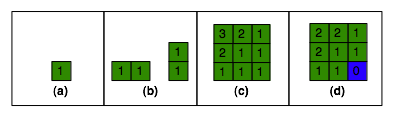
\includegraphics[scale=0.5]{diagrams/calculatingclearance.png}
        \end{center}
        \label{aha-fig:calculatingclearance}
\end{figure}

Although this approach is highly effective, it breaks down when there are multiple terrain types near some location. If we have large agents for example some may be able to traverse the tile and surrounding area while others not. For this reason, probabilistic roadmap methods using clearance are always limited to a single terrain type in the literature. To overcome this problem we propose embedding several clearance values at each fixed point in the environment, each one measuring the nearest-obstacle distance for every type of agent capability.  Capability in this case simply refers to a set of the available terrain types found in our grid environment. Furthermore, we will henceforth refer to agents that can traverse several types of terrain as \emph{multi-capable}.

The process for calculating capability clearances is identical to that described until now with only one minor difference: we need to specify a target capability which we use to calculate the right clearance value. During processing, any tile we encounter that is not traversable for the given capability we will refer to as a \emph{soft obstacle} and assign it a clearance value of 0 for that capability. Tiles which are not traversable by any capability are said to be \emph{hard obstacles} and always assigned 0.  We continue in this manner for each available capability until all map tiles have been processed. Figure \ref{aha-fig:annotations} shows the results of different clearance value annotations we embedded into a tiny map during development.

Using these definitions, we can easily derive the following recursive algorithm for computing clearance annotations:
\begin{equation}
CV(t,c) = min(CV(t_{East}, c), CV(t_{South}, c), CV(t_{Southeast}), c) + BaseClearance
\labe{aha-alg:cv}
\end{equation}
Where $t$ is a traversable tile in our grid map, $CV$ is the clearance value function, $c$ is our target capability and $t_{East}$, $t_{South}$ and $t_{Southeast}$ are also tiles in our grid map (not necessarily traversable); their  subscripts indicate they are octile neighbours of $t$ in the stated directions.

\begin{figure}[htbp]
        \caption{\emph{Single terrain and multi-terrain clearance value annotations.} Top: Clearance values for the single-terrain case. Bottom: Multi-terrain (Plains + Forests) annotations. In both cases, clearance values for hard-obstacles (here, water tiles) is omitted.}
        \begin{center}
                        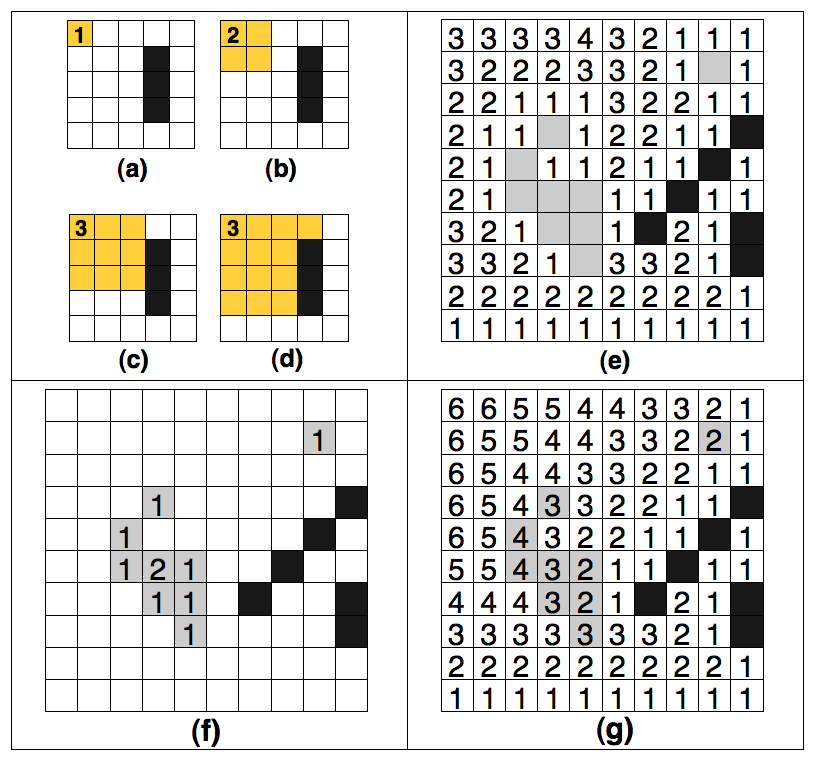
\includegraphics[scale=0.8]{diagrams/annotations.png}
        \end{center}
        \label{aha-fig:annotations}
\end{figure}

If we assume a capability exists for each combination of available terrain types, the exact number of annotations required for each map node is given by:
\begin{equation}
2^(t)/2 - |N_{HO}|
\label{aha-eq:cv}
\end{equation}

Where $t$ is the number of terrains on the map and $N_{HO}$ is the set of hard obstacles. \\ \newline
We derive this formula by noting that each node in the grid has a particular terrain type. It logically follows that each tile will only be traversable by a capability which includes the tile's terrain type meaning we do not need to unnecessarily store 0 clearance values. Similarly, we also avoid storing 0 values for hard obstacles.

